\section{Introduction}

\begin{frame}{Relativistic Heavy-Ion Collisions}
\vspace{0.5em}
Why do we study high-energy nuclear physics? \\[0.5em]

\begin{itemize}
    \item  We want to resolve the nuclear structure.
	\item The \alert{Quark-Gluon Plasma} (QGP) provides insights into the physical processes relevant shortly after the Big Bang.
	\item Particle colliders such as the \alert{LHC} or the \alert{RHIC} are built to reach high energies.
	\item Collision events offer a fruitful playground for testing \alert{QCD} and \alert{statistical models} (focus of this talk/seminar).	
\end{itemize}
\begin{figure}[H]
\centering
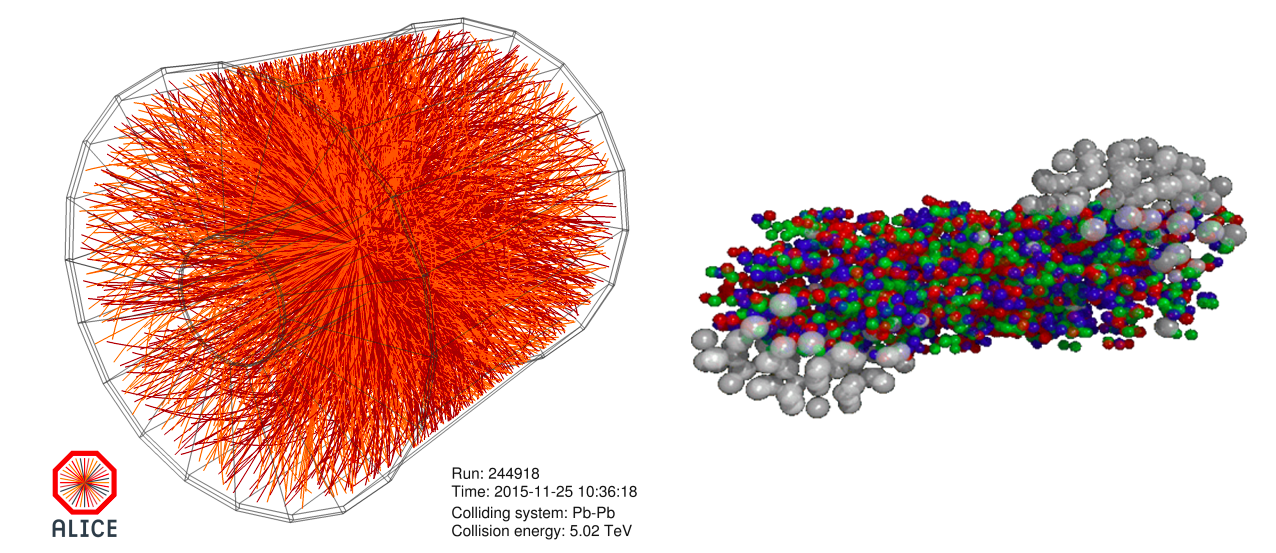
\includegraphics[width = 0.6\textwidth]{figures/introduction}
\caption{Visualization of a Pb-Pb collision event in the ALICE detector at the LHC.\footnotemark}	
\end{figure}
\footnotetext{Source: \tiny{\url{https://www.physi.uni-heidelberg.de/~reygers/lectures/2019/qgp/qgp_lecture_ss2019.html} (23.06.2020)}}
\end{frame}
%TODO: More on history??

\begin{frame}{The different Phases of RHICs}
\begin{figure}[H]
\centering
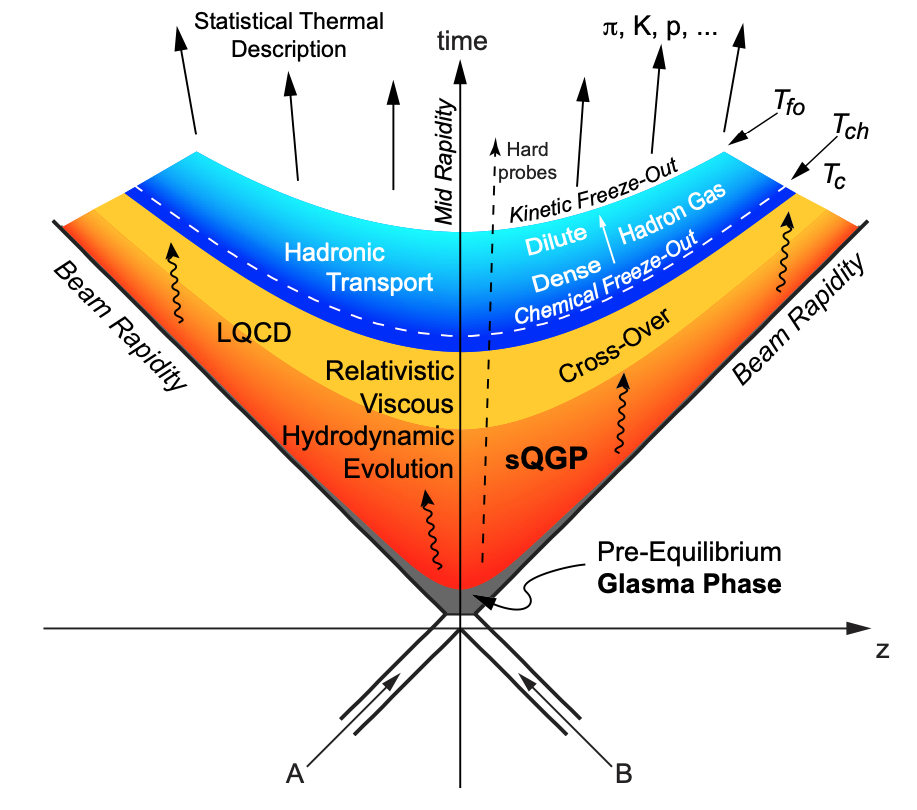
\includegraphics[width = 0.6\textwidth]{figures/rhic_schematic}
\caption{Visualization of the spacetime evolution of the system created in RHICs.\footnotemark \\ In this talk, we will have a closer look at the \alert{pre-equilibrirum} phase (gray area).}	
\end{figure}
\footnotetext{Figure taken from B. Hippolyte's slides: \tiny{\url{http://www.nupecc.org/presentations/hippo_mar17.pdf} (23.06.2020)}}
\end{frame}

%TODO: Phase diagram of QCD Bild??



